\documentclass[12pt, twoside]{article}
\documentclass[12pt, twoside]{article}
\usepackage[letterpaper, margin=1in, headsep=0.2in]{geometry}
\setlength{\headheight}{0.6in}
%\usepackage[english]{babel}
\usepackage[utf8]{inputenc}
\usepackage{microtype}
\usepackage{amsmath}
\usepackage{amssymb}
%\usepackage{amsfonts}
\usepackage{siunitx} %units in math. eg 20\milli\meter
\usepackage{yhmath} % for arcs, overparenth command
\usepackage{tikz} %graphics
\usetikzlibrary{quotes, angles}
\usepackage{graphicx} %consider setting \graphicspath{{images/}}
\usepackage{parskip} %no paragraph indent
\usepackage{enumitem}
\usepackage{multicol}
\usepackage{venndiagram}

\usepackage{fancyhdr}
\pagestyle{fancy}
\fancyhf{}
\renewcommand{\headrulewidth}{0pt} % disable the underline of the header
\raggedbottom
\hfuzz=2mm %suppresses overfull box warnings

\usepackage{hyperref}
\usepackage{float}

\fancyhead[LE]{\thepage}
\fancyhead[RO]{\thepage \\ First and last name: \hspace{2.5cm} \,\\ Section: \hspace{2.5cm} \,}
\fancyhead[LO]{BECA/Huson/Geometry: Similarity \\* 4 December 2024}

\begin{document}
\subsubsection*{3.17 PreTest: Dilation and similarity}
\begin{enumerate}[itemsep=0.5cm]
\item Given $\overline{DEF}$, $DE=7 $, and $EF= 2 \frac{1}{3}$. Find ${DF}$. \par \bigskip
  \begin{tikzpicture}`'
    \draw [-, thick] (1,0)--(7,0);
    \draw [fill] (1,0) circle [radius=0.05] node[below]{$D$};
    \draw [fill] (5,0) circle [radius=0.05] node[below]{$E$};
    \draw [fill] (7,0) circle [radius=0.05] node[below]{$F$};
  \end{tikzpicture}  \vspace{1cm}

\item Point $G$ bisects $\overline{FH}$, with $FG=5x + 2$, $GH=17$. Find $x$. \par \medskip
  \begin{tikzpicture}
      \draw[fill] (0,0) circle [radius=0.05] node[below]{$F$};
      \draw[-, thick] (0,0)--(8,0);
      \draw[fill] (4,0) circle [radius=0.05] node[below]{$G$};
      \draw[fill] (8,0) circle [radius=0.05] node[below]{$H$};
      \node at (2,0.5) [above]{$5x + 2$};
      \node at (6,0.5) [above]{$17$};
      \draw (1.8,-0.2)--(1.9,0.2);
      \draw (2.1,-0.2)--(2.2,0.2);
      \draw (5.8,-0.2)--(5.9,0.2);
      \draw (6.1,-0.2)--(6.2,0.2);
  \end{tikzpicture} \vspace{4cm}

\item Bisect the given angle. \vspace{2cm}
  \begin{center}
  \begin{tikzpicture}[rotate=-60]
    \draw [<->, thick] (80:6)--(0,0)--(20:6);
    \draw [fill] (0,0) circle [radius=0.05] node[below]{$A$};
  \end{tikzpicture}
  \end{center} \vspace{0.5cm}

\newpage
\item Construct a perpendicular to $\overline{AB}$ though $C$.\\
%\hspace{1cm} Given the line  $l$ and point $P$.
  \vspace{1cm}
  \begin{center}
  \begin{tikzpicture}[rotate=-30]
    \draw [<->, thick] (0,0)--(11,0)--(6,-3)--cycle;
    \draw [fill] (0,0) circle [radius=0.05] node[left]{$A$};
    \draw [fill] (11,0) circle [radius=0.05] node[right]{$B$};
    \draw [fill] (6,-3) circle [radius=0.05] node[above right]{$C$};
  \end{tikzpicture}
  \end{center} \vspace{3cm}

\item Apply a clockwise rotation of $90^\circ$ centered at the origin to $\triangle ABC$. Plot and label the image on the axes below.
  \begin{flushright}
    \begin{tikzpicture}[scale=.48]
      \draw [help lines] (-8,-8) grid (8,8);
      \draw [thick, <->] (-8.4,0) -- (8.4,0) node [right] {$x$};
      \draw [thick, <->] (0,-8.4)--(0,8.4) node [above] {$y$};
      \draw [thick]
        (1,2) node[below left] {$A$}--
        (5,5) node[right] {$B$}--
        (6,2) node[below] {$C$}--
        cycle;
    \end{tikzpicture}
  \end{flushright}

\newpage
\item  Reflect $\triangle ABC$ across the $y$-axis. Label the image $\triangle A'B'C'$ on the graph.
  \begin{center}
    \begin{tikzpicture}[scale=0.7]
      \draw [help lines] (-8,-7) grid (8,7);
      \draw [thick, <->] (-8.4,0) -- (8.4,0) node [below right] {$x$};
      \draw [thick, <->] (0,-7.4)--(0,7.4) node [left] {$y$};
      \draw [thick] (-2,3) node[left] {$A$}--
        (3,-4) node[right] {$B$}--
        (4,5) node[above right] {$C$}--
        cycle;
    \end{tikzpicture}
    \end{center}

\item A translation is applied to $\triangle ABC$ moving it to the left 4 and down 3.
\begin{enumerate}
  \item Write as coordinate pairs the vertices of the image, $\triangle A'B'C'$ \\[0.3cm]
  $A(3,-4) \rightarrow$ \\[0.7cm]
  $B(5,-3) \rightarrow$ \\[0.7cm]
  $C(0,2) \rightarrow$ %\\[0.2cm]
  \item Which triangle is larger, or are they the same size? Justify your answer.
\end{enumerate} \vspace{2cm}


\item A translation maps $D(1,4) \rightarrow D'(4,-1)$. What is the image of $E(-2,-3)$ under the same translation? \vspace{2cm}


\newpage

\item Reflect $\triangle ABC$ across the $y$-axis. Then, dilate $\triangle A'B'C'$ by a factor of k = 1.5 centered at the origin to produce $\triangle A''B''C''$. Plot and label the two triangles in the graph below.
\begin{center}
  \begin{tikzpicture}[scale=.7]
    \draw [help lines] (-8,-6) grid (8,8);
    \draw [thick, <->] (-8.4,0) -- (8.4,0) node [right] {$x$};
    \draw [thick, <->] (0,-6.4)--(0,8.4) node [above] {$y$};
    \draw [thick]
      (0,0) node[below left] {$A$}--
      (4,4) node[right] {$B$}--
      (4,2) node[below] {$C$}--
      cycle;
  \end{tikzpicture}
\end{center}

\begin{multicols}{2}
[\item A dilation maps $\triangle ABC \rightarrow \triangle DEF$, with $AB=10$, $BC=12$, $AC=5$, and $DF=6$.] \vspace{0.5cm}
  \begin{tikzpicture}[scale=1.2]
    \coordinate [label=above left:$B$](A) at (110:2.5);
    \coordinate [label=below:$A$](B) at (0, 0);
    \coordinate [label=below:$C$](C) at (0:1.5);
    \draw [thick] (A)--(B)--(C)--cycle;
    \draw [thick, xshift=2.5cm, yshift=0cm, scale=1.25, rotate=0] (110:2.5) node[above]{$E$}--
    (0,0) node[below]{$D$}--
    (0:1.5) node[below]{$F$}--cycle;
    \node at (110:1.25)[left]{$10$};
    \node at (55:1.6)[left]{$12$};
    \node at (0:0.75)[below]{$5$};
    \node at (0:3.5)[below]{$6$};
  \end{tikzpicture}\\
  Find the scale factor and missing sides.
  \begin{enumerate}
    \item $\displaystyle k=$ \vspace{0.5cm}
    \item $\displaystyle DE=$ \vspace{0.5cm}
    \item $EF=$
  \end{enumerate}
\end{multicols} \vspace{1cm}
    
\newpage
\item Dilate the triangle $ABC \rightarrow A'B'C'$ by a factor of $k=1.5$ centered at the origin.
  \begin{multicols}{2}
    \begin{tikzpicture}[scale=.7]
      \draw [help lines] (-4,-4) grid (6,5);
      \draw [thick, ->] (-4.2,0) -- (6.4,0) node [below right] {$x$};
      \draw [thick, ->] (0,-4.2)--(0,5.4) node [left] {$y$};
      \draw [thick] (-2,0)node[below left]{$A$}--
        (2,-2)node[right]{$C$}--
        (4,2)node[below right]{$B$}--cycle;
    \end{tikzpicture}

    Complete the table of coordinate mappings.\\[0.5cm]
    $A(-2,0) \rightarrow A'(-3,0)$ \vspace{3cm}
  \end{multicols}

\item Given $\triangle USA \sim \triangle MEX$ and $m\angle U =60^\circ$, $m\angle A =85^\circ$. Find the remaining angle measures.
\begin{flushright}
    \begin{tikzpicture}[scale=0.9]
    \coordinate [label=above left:$S$](A) at (60:3);
    \coordinate [label=left:$U$](B) at (0, 0);
    \coordinate [label=below:$A$](C) at (0:1.75);
    \draw [thick] (A)--(B)--(C)--cycle;
    \draw [thick, xshift=7cm, yshift=4cm, scale=1.6, rotate=-170] (60:3) node[left]{$E$}--
    (0,0) node[right]{$M$}--
    (0:1.75) node[above]{$X$}--cycle;
  \end{tikzpicture}
\end{flushright}

\item A dilation centered at $A$ with a scale factor of $\displaystyle k=1.75$ maps $\triangle ABC \rightarrow \triangle ADE$. Given $AB=12.4$, $AC=8.8$, $DE=13.3$. 
\begin{multicols}{2}
  Find the remaining side lengths.\\[0.25cm]
  $AD=$\\[1cm]
  $AE=$\\[1cm]
  $BC=$\\
  \begin{flushright}
    \begin{tikzpicture}[scale=1.2]
      \draw [thick]
      (0,0)node[below right]{$A$}--
      (0:7.5)node[below]{$D$}--
      (30:5)node[above]{$E$}--cycle;
      \draw [thick]
      (0:5)node[below]{$B$}--
      (30:3.33)node[above left]{$C$};
      \node at (0:2.5)[below]{$12.4$};
      \node at (15:6)[right]{$13.3$};
      \node at (35:1.7)[above]{$8.8$};
    \end{tikzpicture}
  \end{flushright}
\end{multicols}\vspace{1cm}


\newpage

\item Triangle $ABC$ is dilated with a scale factor of $k=2.5$ centered at $A$, yielding $\triangle ADE$, as shown. Given $AB=6$, $AC=5$, and $DE=17.5$. \\[0.25cm] Find $AD$, $AE$, and $BC$. Then find $BD$ and $CE$.
\begin{flushright}
  \begin{tikzpicture}[scale=0.8]
    \draw [thick]
    (0,0)node[above]{$A$}--
    (-130:8.75)node[below]{$D$}--
    (-60:7.5)node[below]{$E$}--cycle;
    \draw [thick]
    (-130:3.5)node[above left]{$B$}--
    (-60:3)node[above right]{$C$};
    \node at (-150:1.75)[below]{$6$};
    \node at (-55:1.5)[right]{$5$};
    \node at (-95:7.5)[above]{$17.5$};
  \end{tikzpicture}
\end{flushright} \vspace{1cm}

\item A dilation centered at the origin and scale factor $k$ maps $P(2,5) \rightarrow P'(5,12.5)$. Find $k$. \vspace{2cm}


\item In the diagram below, $\triangle ABC \sim \triangle DEF$, $DE=6$, $AB=x$, $AC=2x$, and $DF=2x+4$. Determine the length of $\overline{AB}$.
  \begin{flushright}
    \begin{tikzpicture}[scale=0.9]
    \coordinate [label=above left:$A$](A) at (85:2);
    \coordinate [label=below:$B$](B) at (0, 0);
    \coordinate [label=right:$C$](C) at (-20:3);
      \draw [thick] (A)--(B)--(C)--cycle;
      \node at (95:1)[left]{$x$};
      \node at (35:1.75)[right]{$2x$};
      \draw [thick, xshift=5cm, yshift=0.5cm] (85:3) node[above]{$D$}--
      (0,0) node[below]{$E$}--
      (-20:4.5) node[right]{$F$}--cycle;
      \draw [thick, xshift=5cm, yshift=0.5cm](90:1.5) node[left]{$6$};
      \draw [thick, xshift=5cm, yshift=0.5cm](30:2.75) node[right]{$2x+4$};
  \end{tikzpicture}
  \end{flushright}



\end{enumerate}
\end{document}